\documentclass[final]{siamltex}

% for red MarginPars
\usepackage{color}

% for \boldsymbol
\usepackage{amsmath}
\usepackage{latexsym}
\usepackage{graphicx}
\usepackage{geometry}
\usepackage{hyperref}

% total number of floats allowed on a page
\setcounter{totalnumber}{100}

% float page fractions
\renewcommand{\topfraction}{0.9}
\renewcommand{\bottomfraction}{0.9}
\renewcommand{\textfraction}{0.2}

% MarginPar
\setlength{\marginparwidth}{0.75in}
\newcommand{\MarginPar}[1]{\marginpar{\vskip-\baselineskip\raggedright\tiny\sffamily\hrule\smallskip{\color{red}#1}\par\smallskip\hrule}}

% for non-stacked fractions
\newcommand{\sfrac}[2]{\mathchoice
  {\kern0em\raise.5ex\hbox{\the\scriptfont0 #1}\kern-.15em/
   \kern-.15em\lower.25ex\hbox{\the\scriptfont0 #2}}
  {\kern0em\raise.5ex\hbox{\the\scriptfont0 #1}\kern-.15em/
   \kern-.15em\lower.25ex\hbox{\the\scriptfont0 #2}}
  {\kern0em\raise.5ex\hbox{\the\scriptscriptfont0 #1}\kern-.2em/
   \kern-.15em\lower.25ex\hbox{\the\scriptscriptfont0 #2}}
  {#1\!/#2}}

\def\Ab {{\bf A}}
\def\bb {{\bf b}}
\def\Fb {{\bf F}}
\def\gb {{\bf g}}
\def\vb {{\bf v}}
\def\Wb {{\bf W}}
\def\xb {{\bf x}}

\def\deltab {\boldsymbol{\delta}}
\def\Psib   {\boldsymbol{\Psi}}
\def\Sigmab {\boldsymbol{\Sigma}}
\def\taub   {\boldsymbol{\tau}}

\def\half   {\frac{1}{2}}
\def\myhalf {\sfrac{1}{2}}

\begin{document}

%==========================================================================
% Title
%==========================================================================
\title{Implicit Low Mach Number Binary Mixing Notes}

\maketitle

\section{Equations}
We have two incompressible fluids with densities $\bar\rho_1$ and $\bar\rho_2$, where 
each fluid does not change volume upon mixing.  Defining $\rho$ to be the density of
a mixture of these fluids, the densities of each fluid are $\rho_1 \equiv \rho c$ and 
$\rho_2 \equiv \rho(1-c)$, where $c$ is the {\it mass} fraction of the first fluid.  
Thus, $\rho = \rho_1 + \rho_2$.  Since the fluids do not change volume upon mixing, 
the equation of state will enforce that the {\it volume} fractions must sum to 1:
\begin{equation}
\frac{\rho_1}{\bar\rho_1} + \frac{\rho_2}{\bar\rho_2} =
\frac{\rho c}{\bar\rho_1} + \frac{\rho(1-c)}{\bar\rho_2} = 1 
\quad \rightarrow \quad
\rho = \left(\frac{c}{\bar\rho_1} + \frac{1-c}{\bar\rho_2}\right)^{-1}.
\end{equation}
The isothermal low Mach number equations of motion are:
\begin{eqnarray}
\partial_t\rho &=& -\nabla\cdot(\rho\vb),\\
\partial_t\rho_1 &=& -\nabla\cdot(\rho_1\vb) + \underbrace{\nabla\cdot\rho\chi\nabla c + \nabla\cdot\Psib}_{\nabla\cdot\Fb},\\
\partial_t(\rho\vb) &=& -\nabla\cdot(\rho\vb\vb^T) - \nabla\pi + \mathcal{A}_0\vb + \nabla\cdot\Sigmab + \rho\gb,
\end{eqnarray}
subject to
\begin{equation}
\nabla\cdot\vb = S \equiv \underbrace{\left(\frac{1}{\bar\rho_1}-\frac{1}{\bar\rho_2}\right)}_{-(\rho^{-1}\beta)}\nabla\cdot\Fb.
\end{equation}
Thus, $S \equiv S(\Fb)$.  The stochastic terms are:
\begin{eqnarray}
\Psib &=& \sqrt{\frac{2\chi\rho\mu_c^{-1}k_BT}{\Delta t\Delta V}}\widetilde\Wb,\label{eq:rho1 stoch}\\
\Sigmab &=& \sqrt{\frac{\eta k_B T}{\Delta t\Delta V}}\left(\Wb + \Wb^T\right),\label{eq:mom stoch}
\end{eqnarray}
where $\Wb$ and $\widetilde\Wb$ are standard white-noise random Gaussian tensor
and vector fields with uncorrelated components.  In our implementation, 
we use an ideal gas mixture for (\ref{eq:rho1 stoch}) with $\mu_c^{-1}k_BT \equiv c(1-c)$ so that
\begin{equation}
\Psib = \sqrt{\frac{2\chi\rho c(1-c)}{\Delta t\Delta V}}\widetilde\Wb
\end{equation}
Also, in (\ref{eq:mom stoch}) we use
\begin{equation}
\widehat\Wb = \sqrt{2}\left(\Wb + \Wb^T\right) \quad \rightarrow \quad
\Sigmab = \sqrt{\frac{2\eta k_B T}{\Delta t\Delta V}}\widehat\Wb,
\end{equation}
where $\widehat\Wb$ is a symmetric Gaussian random tensor field, and the
extra factor of $\sqrt{2}$ accounts for the reduction in variance due to the averaging.\\

The code has several options for the viscous stress tensor.  For ease of exposition,
we define $\mathcal{A}_0$ as a function of a velocity vector, $\vb$ (the superscript
for $\mathcal{A}_0$ indicates the temporal discretization for the transport coefficients):\\
\begin{itemize}
\item $|${\tt visc\_type}$|$=1 $\quad\rightarrow\quad \mathcal{A}_0^n\vb \equiv \nabla\cdot\beta^n\nabla\vb$.\\
\item $|${\tt visc\_type}$|$=2 $\quad\rightarrow\quad \mathcal{A}_0^n\vb \equiv \nabla\cdot\left\{\beta^n[\nabla\vb + (\nabla\vb)^T]\right\}$.\\
\item $|${\tt visc\_type}$|$=3 $\quad\rightarrow\quad \mathcal{A}_0^n\vb \equiv \nabla\cdot\left\{\beta^n[\nabla\vb + (\nabla\vb)^T] + \mathcal{I}\left(\gamma^n - \frac{2}{3}\beta^n\right)(\nabla\cdot\vb)\right\}$.\\
\end{itemize}

\section{GMRES Solver}
We also have a standalone GMRES solver of the form,
\begin{equation}
\underbrace{
\left(\begin{array}{cc}
\mathcal{A} & \mathcal{G} \\
-\mathcal{D} & 0
\end{array}\right)
}_{\Ab}
\underbrace{
\left(\begin{array}{c}
\xb_{\vb} \\
x_p
\end{array}\right)
}_{\xb}
=
\underbrace{
\left(\begin{array}{c}
\bb_{\vb}\\
b_p
\end{array}\right)}_{\bb},
\end{equation}
where $\xb_\vb$ and $\bb_\vb$ are staggered quantities and $x_p$ and $b_p$ are
cell-centered quantities.  The gradient operator, $\mathcal{G}$, operates on
cell-centered data and returns a staggered field.  The divergence operator, 
$\mathcal{D}$, operates on staggered data and returns a cell-centered field.  
The Helmholtz-like operator, $\mathcal{A}$, has the general form,
$\mathcal{A} = \Theta\alpha\mathcal{I} - \mathcal{A}_0$, where
$\Theta$ is a constant parameter,
$\alpha$ is a cell-centered quantity,
$\mathcal{I}$ is the identity matrix, 
and $\mathcal{A}_0$ represents the viscous stress tensor.
Both $\mathcal{A}$ and $\mathcal{A}_0$ operate on staggered data and return
a staggered field.\\

\section{Algorithm}
Here is the time-advancement scheme.\\ \\
{\bf Step 0: Initialization:}\\

Initialize $\vb^{\rm init}, \rho^0, \rho_1^0, \chi^0, \eta^0, \kappa^0$, and $\pi^0$.
Then, perform projection to obtain an initial velocity field, $\vb^0$, that satisfies
\begin{equation}
\nabla\cdot\vb^0 = S(\Fb^0); \qquad 
\Fb^0 = (\rho\chi\nabla c)^0 + \underbrace{\sqrt{\frac{2\left[\chi\rho c(1-c)\right]^0}{\Delta t\Delta V}}\widetilde\Wb^0}_{\Psib^0}.
\end{equation}
We do this by solving for $\phi$ and updating $\vb^{\rm init}$ as follows:
\begin{equation}
\nabla\cdot\frac{1}{\rho^0}\nabla\phi = \nabla\cdot\vb^{\rm init} - S^0,
\end{equation}
\begin{equation}
\vb^0 = \vb^{\rm init} - \frac{1}{\rho}\nabla\phi.
\end{equation}
{\bf Step 1: Forward Euler Scalar Predictor:}
\begin{eqnarray}
\rho^{*,n+1} &=& \rho^n + \Delta t\nabla\cdot(-\rho^n\vb^n),\\
\rho_1^{*,n+1} &=& \rho_1^n + \Delta t\nabla\cdot(-\rho_1^n\vb^n + \Fb^n),
\end{eqnarray}
with
\begin{equation}
\Fb^n = (\rho\chi\nabla c)^n + \underbrace{\sqrt{\frac{2\left[\chi\rho c(1-c)\right]}{\Delta t\Delta V}}\widetilde\Wb^n}_{\Psib^n}.
\end{equation}
Note that $\Fb^n$ has already been computed during {\bf Step 4} of the previous time step
(or the initialization {\bf Step 0} if $n=0$).\\ \\
{\bf Step 2: Crank-Nicolson Velocity Predictor:}\\ \\
First, define
\begin{equation}
S^{*,n+1} \equiv S(\Fb^{*,n+1});
\qquad
\Fb^{*,n+1} = (\rho\chi\nabla c)^{*,n+1} + \Psib^n.
\end{equation}
Then, define $\vb^{*,n+1} = \vb^n + \deltab\vb, \pi^{*,n+1} = \pi^n + \delta\pi$ and solve
for $\deltab\vb$ and $\delta\pi$:
\begin{eqnarray}
\frac{\rho^{*,n+1}(\vb^n + \deltab\vb) - \rho^n\vb^n}{\Delta t} + \nabla(\pi^n+\delta\pi) &=&\nonumber\\
&&\hspace{-1.5in}\nabla\cdot(-\rho^n\vb^n\vb^n) + \half\left[\mathcal{A}_0^n\vb^n + \mathcal{A}_0^{*,n+1}(\vb^n + \deltab\vb)\right] + \nabla\cdot\underbrace{\sqrt{\frac{2\eta^n k_B T}{\Delta t\Delta V}}\widehat\Wb^n}_{\Sigmab^n}.
\end{eqnarray}
\begin{equation}
\nabla\cdot(\vb^n+\deltab\vb) = S^{*,n+1}.
\end{equation}
We rewrite this system as
\begin{eqnarray}
\left(\frac{\rho^{*,n+1}}{\Delta t} - \half\mathcal{A}_0^{*,n+1}\right)\deltab\vb + \nabla\delta\pi &=& \frac{(\rho^n-\rho^{*,n+1})\vb^n}{\Delta t} -\nabla\pi^n\nonumber\\
&&\hspace{-0.5in}+ \nabla\cdot(-\rho^n\vb^n\vb^n) + \half\left(\mathcal{A}_0^n\vb^n + \mathcal{A}_0^{*,n+1}\vb^n\right) + \nabla\cdot\Sigmab^n,\label{eq:CN Vel Pred}
\end{eqnarray}
\begin{equation}
-\nabla\cdot\deltab\vb = \nabla\cdot\vb^n - S^{*,n+1}.
\end{equation}
Relating this to the GMRES solver, we can see that we are solving for 
$(\xb_\vb,x_p) = (\deltab\vb,\delta\pi)$ with $b_p = \nabla\cdot\vb^n-S^{*,n+1}$ (note the change in sign!) 
and $\bb_\vb$ equal to the right-hand-side of (\ref{eq:CN Vel Pred}).  For the Helmholtz-like operator, 
$\mathcal{A}=\Theta\alpha\mathcal{I} - \mathcal{A}_0$, we have $\Theta=1/\Delta t, \alpha=\rho^{*,n+1}, 
\beta=\eta/2$, and $\gamma=\kappa/2$.\\ \\
{\bf Step 3: Trapezoidal Scalar Corrector:}
\begin{eqnarray}
\rho^{n+1} &=& \half\rho^n + \half\left[\rho^{*,n+1} + \Delta t\nabla\cdot(-\rho^{*,n+1}\vb^{*,n+1})\right],\\
\rho_1^{n+1} &=& \half\rho_1^n + \half\left[\rho_1^{*,n+1} + \Delta t\nabla\cdot(-\rho_1^{*,n+1}\vb^{*,n+1} + \Fb^{*,n+1})\right].
\end{eqnarray}
Note that $\Fb^{*,n+1}$ has already been computed during {\bf Step 2}.\\ \\
{\bf Step 4: Crank-Nicolson Velocity Corrector:}\\ \\
First, define
\begin{equation}
S^{n+1} \equiv S(\Fb^{n+1});
\qquad
\Fb^{n+1} = (\rho\chi\nabla c)^{n+1} + \underbrace{\sqrt{\frac{2\left[\chi\rho c(1-c)\right]^{n+1}}{\Delta t\Delta V}}\widetilde\Wb^{n+1}}_{\Psib^{n+1}}.
\end{equation}
Note the use of time-advanced stochastic concentration fluxes for use in $S$.  Finally, 
define $\vb^{n+1} = \vb^n + \deltab\vb$ and $\pi^{n+1} = \pi^n + \delta\pi$ and
solve the following system for $(\deltab\vb,\delta\pi)$:
\begin{eqnarray}
\left(\frac{\rho^{n+1}}{\Delta t} - \half\mathcal{A}_0^{n+1}\right)\deltab\vb + \nabla\delta\pi &=& \frac{(\rho^n-\rho^{n+1})\vb^n}{\Delta t} -\nabla\pi^n\nonumber\\
&&\hspace{-1.25in}+ \half\nabla\cdot(-\rho^n\vb^n\vb^n - \rho^{n+1}\vb^{*,n+1}\vb^{*,n+1}) + \half\left(\mathcal{A}^n_0\vb^n + \mathcal{A}^{n+1}_0\vb^n\right) + \nabla\cdot\Sigmab^n,
\end{eqnarray}
\begin{equation}
-\nabla\cdot\deltab\vb = \nabla\cdot\vb^n - S^{n+1}.
\end{equation}

\section{Boundary Conditions}
The types of non-periodic, ``physical'' boundary conditions we consider are 
(i) no-slip impermeable walls,
(ii) free-slip impermeable walls,
(iii) no-reservoir, and
(iv) free-slip reservoir conditions.
We impose boundary conditions on the primitive variables and velocities,
i.e., $\rho,c$, and $\vb$.\\

{\bf No-Slip Wall:}  For impermeable walls, there can be no diffusive
flux, $F_n=0$, and zero advective flux, $\rho v_n = \rho_1 v_n = 0$.  The zero
diffusive flux implies a homogeneous Neumann condition on $c$, and also $\rho$ since it
can be derived from $c$ and the EOS.  The zero advective flux implies that $v_n=0$ on the
boundary.  The no-slip condition implies that each $v_{\tau}=0$ on the boundary.\\

{\bf Free-Slip Impermeable Wall:}  This is the same situation as the no-slip impermeable
wall, except that the tangential velocities is subject to the condition that the
tangential compoment of the normal viscous stres vanishes.  In other words, for each 
tangential direction $\tau$,
\begin{equation}
\eta\left(\frac{\partial v_n}{\partial\tau} + \frac{\partial v_{\tau}}{\partial n}\right) = 0.\label{eq:free slip}
\end{equation}
Note that for impermeable walls, $v_n=0$ and therefore we simply require $\partial v_{\tau}/\partial n=0$.\\

{\bf No-Slip Reservoir:} We specify $c$ with a Dirichlet condition at the boundary, 
and use the EOS to obtain $\rho$ at the
boundary.  The normal velocity must be equal to $-(\rho^{-1}\beta)F_n$ in order for
the EOS to remain satisfied.  The no-slip condition implies that each $v_{\tau}=0$ on the 
boundary.\\

{\bf Free-Slip Reservoir:} This is the same situation as the no-slip reservoir, except
that each $v_{\tau}$ is subject to (\ref{eq:free slip}).  Since in general
the normal velocity is not constant, we will have an inhomogeneous neumann condition
on each $v_{\tau}$.

\subsection{Implementation}

\subsubsection{Primitive Variables}
For all physical boundaries, the value of a primitive
variable on the boundary shall be stored in the ghost cell for convenience.  This
is true regardless of whether we use a homogeneous Neumann or Dirichlet condition.
For homogeneous Neumann, we simply copy the interior cell value, thus representing
a first-order extrapolation.  For Dirichlet conditions, we prescribe $c$ and use
the EOS to obtain $\rho$.  Note that the transport coefficients, $(\eta,\kappa,\chi)$,
are functions of the primitive variables, so when we compute them, we simply loop
over valid {\it and} ghost cells, and do not require special routines to fill
the ghost cells aftewards.

\subsubsection{Velocities}
%%%%%%%%%%%%%%%%%%%%%%%%%%%%%%%%%
\begin{figure}[tb]
\centering
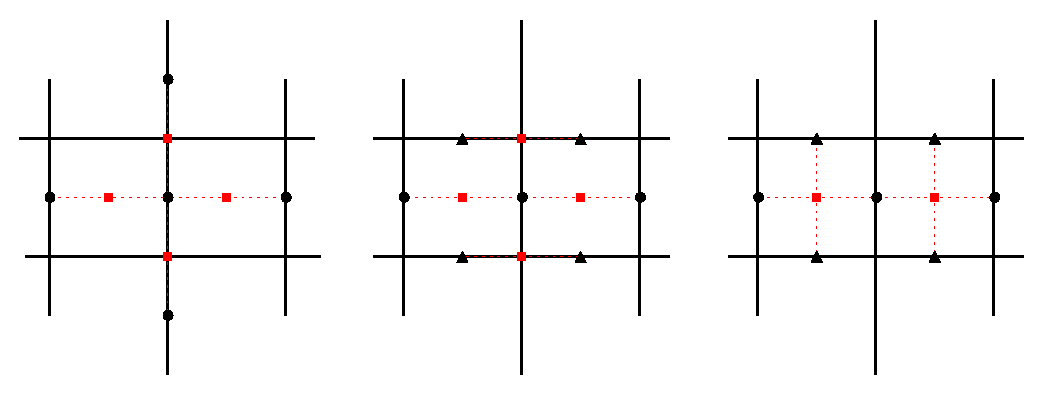
\includegraphics[width=5.25in]{viscOp}
\caption{The stencils for the $x$-component of (Left) $\nabla\cdot\beta\nabla\vb$, (Middle) 
$\nabla\cdot\beta(\nabla\vb)^T$, and (Right) $\nabla\cdot[\mathcal{I}(\gamma-\frac{2}{3}\beta)(\nabla\cdot\vb)]$.  
The black circles indicate locations of $u$.
The black triangles indicate locations of $v$.
The red dots indicate the location of the $\beta$ and the gradients of velocity.}\label{fig:viscOp}
\end{figure}
%%%%%%%%%%%%%%%%%%%%%%%%%%%%%%%%%
%%%%%%%%%%%%%%%%%%%%%%%%%%%%%%%%%
\begin{figure}[tb]
\centering
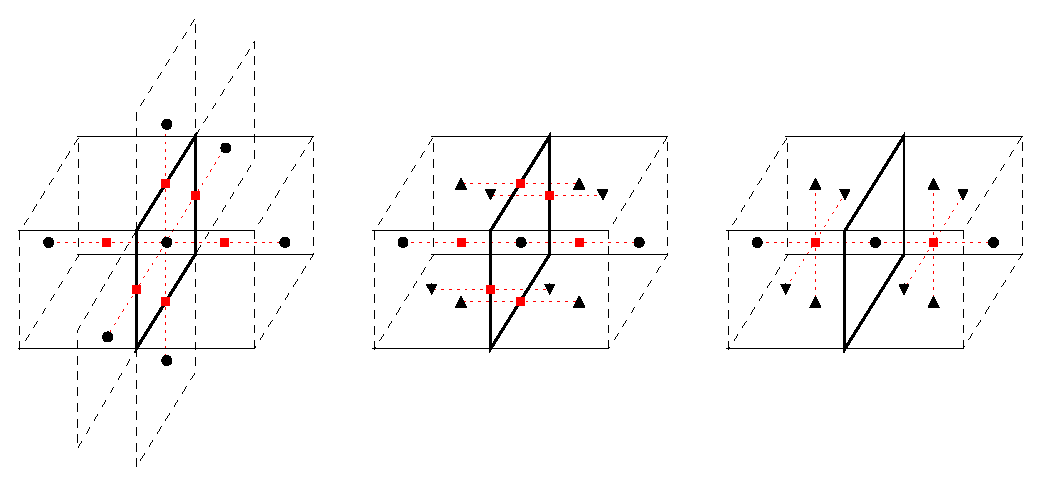
\includegraphics[width=5.25in]{viscOp_3d}
\caption{The stencils for the $x$-component of (Left) $\nabla\cdot\beta\nabla\vb$, (Middle) 
$\nabla\cdot\beta(\nabla\vb)^T$, and (Right) $\nabla\cdot[\mathcal{I}(\gamma-\frac{2}{3}\beta)(\nabla\cdot\vb)]$.  
The black circles indicate locations of $u$.
The black triangles indicate locations of $v$ and $w$.
The red dots indicate the location of the $\beta$ and the gradients of velocity.}\label{fig:viscOp_3d}
\end{figure}
%%%%%%%%%%%%%%%%%%%%%%%%%%%%%%%%%
It is helpful to first consider the stencils for the viscous operators, as illustrated
in Figures \ref{fig:viscOp} and \ref{fig:viscOp_3d} for two and three dimensions.
There are a few key design principles to keep in mind:
\begin{itemize}
\item The evaluation of the viscous operator for faces {\it on} the boundary must
evaluate to zero, so it does not matter what value is stored for the normal component
of velocity in the ghost face outside of the valid region, unless you are concerned 
about possible intermediate {\tt NaN} states that will later be overwritten.
\item The value of the normal velocity {\it on} the boundary {\it does} matter, since it
enters the stencil for the first interior normal velocity face.
\item The value of transverse velocities in ghost faces behind physical boundaries
{\it does} matter, so we make sure to fill them using the appropriate physical 
boundary condition.
\item When setting normal velocities on physical boundaries, we don't have to worry
about corner ghost faces.  Those only matter if we are periodic in the transverse
direction, in which case the call to {\tt multifab\_physbc} should take care of them.
\item When setting transverse velocity ghost faces behind physical boundaries, we do
not have to worry about ghost faces that are outside the valid region with respect
to the problem domain in the transverse direction.  Those only matter if we are 
periodic in the transverse direction, in which case the call to {\tt multifab\_physbc} 
should take care of them.
\end{itemize}

We have two subroutines that deal with velocity boundary conditions.  Each of these
take in an optional multifab argument that represents the Dirichlet value on the
boundary.  Note that ``Dirichlet'' here can either refer to the prescribed value
of normal velocity on the boundary, or a Dirichlet velocity {\it or} traction
condition used to determine the ghost face values for transverse velocity.
If no multifab is passed in, it is assumed that the boundary conditions
are homogeneous.  The subroutine {\tt multifab\_physbc\_domainvel} sets the 
value for faces on the boundary.  The subroutine {\tt multifab\_physbc\_macvel}
sets the transverse velocity ghost faces behind the physical boundary.

For {\tt multifab\_physbc\_domainvel}, the optional multifab that gets passed in
must be face-centered, and requires no ghost cells.

For {\tt multifab\_physbc\_macvel}, the optional multifab that gets passed in
must be face-centered, and in three dimensions each velocity component needs
a separate face-centered multifab (or a multifab with two components) to handle
boundary conditions at each transverse direction.  These multifabs do not requires
ghost cells either.  You could in principle use edge-based multifabs here, but
hopefully the face-centered version will be less confusing.

\end{document}
